\section{Antecedentes y justificación}
\subsection{Estado del arte}
\subsubsection{Diseño Atómico}
El diseño atómico es una metodología de diseño que se centra en la creación
de sistemas de diseño modulares y reutilizables. La idea principal es dividir
las diferentes funcionalidades de un sistemas en sus partes más fundamentales,
de manera que cada una de estas partes pueda ser reutilizada en diferentes
contextos. Este enfoque permite tener un mayor control sobre cada una de las
partes del sistema, facilitando su mantenimiento, documentación y reutilización.
Originalmente, el diseño atómico ha sido aplicado en el diseño de interfaces
de usuario, pero su filosofía puede ser aplicada a cualquier sistema de diseño
modular. En el contexto de este proyecto, el diseño atómico se aplicará al
diseño de un sistema de componentes para el desarrollo de modelos de aprendizaje
automático.\medskip

Dentro del diseño atómico, los componentes se dividen en cinco categorías
principales, que representan diferentes niveles de abstracción. Estas categorías
son: átomos, moléculas, organismos, plantillas y páginas. Cada una de estas
categorías representa un nivel de abstracción diferente, y se relaciona con
las demás categorías de manera jerárquica. La figura \ref{fig:atomic-design}
muestra la estructura tradicional del diseño atómico. 

\begin{figure}[ht]
    \centering
    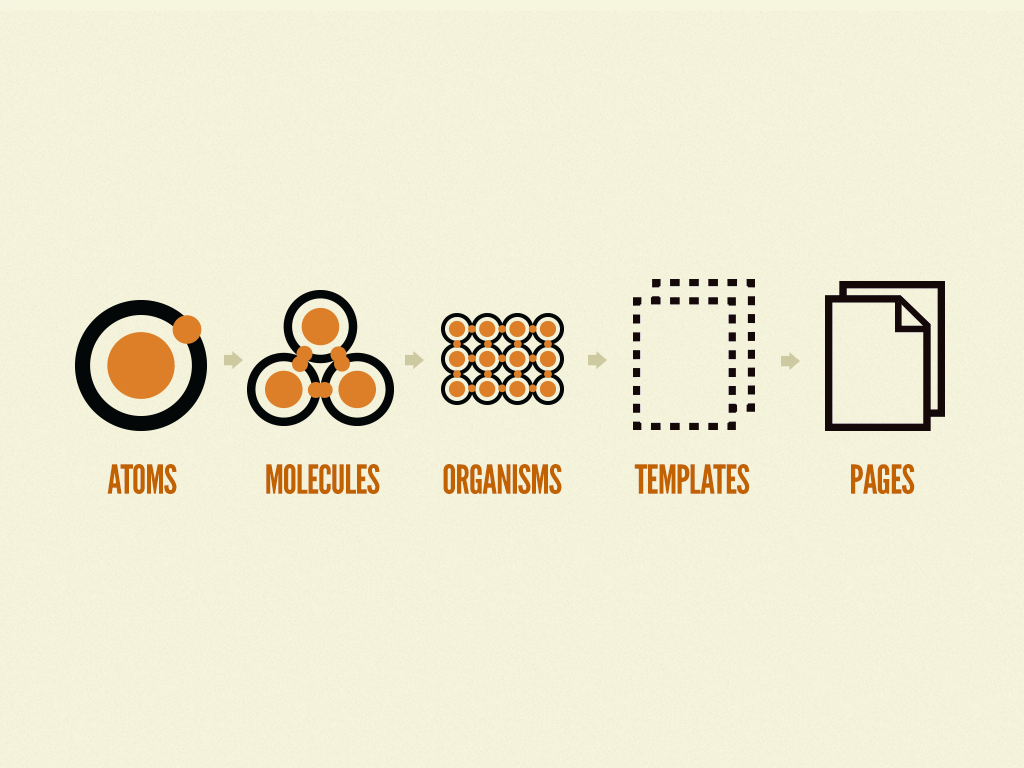
\includegraphics[width=0.7\textwidth]{atomic-design-process.png}
    \caption{Estructura tradicional diseño Atómico}\label{fig:atomic-design}
\end{figure}

A continuación, se describen brevemente cada una de las categorías:
\begin{itemize}
    \item \textbf{Átomos:} Los átomos son los componentes más básicos de un sistema
    de diseño. Representan las funcionalidades más fundamentales, solo tienen
    una responsabilidad y no dependen de otros componentes.
    \item \textbf{Moléculas:} Las moléculas son la combinación de varios átomos
    para formar una funcionalidad más compleja. Representan la combinación de
    diferentes funcionalidades básicas para formar una funcionalidad más compleja.
    \item \textbf{Organismos:} Los organismos son la combinación de varias moléculas
    y átomos para formar una funcionalidad completa.
    \item \textbf{Plantillas:} Las plantillas son la combinación de varios Organismos
    para dar forma a un contenido o funcionalidad completa.
    \item \textbf{Páginas:} Las páginas son la combinación de varias plantillas.
\end{itemize}

Esta estructura jerárquica permite que los componentes sean reutilizados en
diferentes contextos, y que cada uno de ellos pueda ser modificado de manera
independiente. Además, se facilita la documentación y el mantenimiento de los
componentes, ya que cada uno de ellos es independiente de los demás. Podemos
ver multitud de ejemplos de diseño atómico en grandes empresas y que nosotros utilizamos
a diario, como por ejemplo en la creación de sistemas de diseño Microsoft Fluent
Design o Google Material Design entre otros.\medskip

Aunque el diseño atómico se ha aplicado tradicionalmente a la creación de interfaces
de usuario, su filosofía puede ser aplicada a cualquier sistema de diseño modular.
En el contexto de este proyecto, el diseño atómico se aplicará para la creación de un
sistema de componentes en el desarrollo de modelos de aprendizaje automático.
Traeremos la filosofía del diseño atómico y la adaptaremos a nuestro contexto,
con las particularidades y necesidades que requiere el desarrollo de modelos de
aprendizaje automático. 
\subsection{Antecedentes}
\pagebreak